\documentclass[12pt]{article}
\usepackage{fullpage}
\usepackage{nopageno}
\usepackage{setspace}
\usepackage{acronym}
\usepackage{graphicx}
\usepackage{multicol}

\author{Charles Pittman}
\title{AC Circuits}

\acrodef{AC}{Alternating Current}
\acrodef{DC}{Direct Current}
\acrodef{EE}{Electrical Engineering}
\acrodef{EMF}{electromotive force}

%\doublespacing{}
\begin{document}
  \maketitle

  \section*{Introduction}
  The study of electronics generally begins with exploring the function and
  operation of \ac{DC} circuits, with skills learned then translated for
  \ac{AC} circuits.  In that translation some students tend to focus more on
  applying the formulas in problem solving, losing sight of how they were
  derived.  As a result, they may have trouble describing what \ac{AC} is, how
  it functions, or how it's generated.

  \section*{What is \ac{AC}?}
  Because current flows in a single direction in \ac{DC} circuits, the polarity
  of any terminal stays constant.  As the name implies, direction of current
  flow in \ac{AC} circuits alternates, and polarity at terminals with it.
  Figure~\ref{acwave} shows how these values change over time.  One full
  alternation, or period, is marked by the section labeled $T$; the frequency
  of an \ac{AC} waveform refers to the number of periods per second.

  The horizontal axis in Figure~\ref{acwave} can be measured in time, degrees,
  or radians.  One cycle of a sinusoidal wave is $360^\circ$ or $2\pi$ radians.
  This figure also illustrates phase angle, either as the time delay between
  two waveforms or as the angle between them.

  This time difference is also what is being referred to when a waveform is
  described as either ``leading'' or ``lagging'' another.  With respect to a
  reference, a leading waveform is one that is further along in its cycle.

  \section*{How is \ac{AC} Generated?}
  Figure~\ref{alternator} shows a simple model of a three-phase alternator,
  consisting of a magnetic rotor and stator with three separate sets of coil
  windings mounted 120$^\circ$ from each other.  In accordance with Faraday's
  law of induction, an \ac{EMF} is created in the conductors as the magnetic
  field rotates with the shaft, with each set of windings as a separate phase.

  Not surprisingly, most values used in solving \ac{AC} circuits describe the
  characteristics of the alternator.  The period previously mentioned is one
  revolution of the rotor, so the frequency of the \ac{AC} waveform produced is
  the number of revolutions per second.

  \section*{What is Complex Power?}
  Impedance, the opposition of current in a circuit, is extended in \ac{AC}.
  The fields in capacitors and inductors continue to grow in \ac{DC} circuits
  until large enough to stop current and voltage, respectively.  They function
  similarly in \ac{AC} circuits, but discharge each time current changes
  direction.

  The sum of capacitance and inductance, referred to as reactance, describes
  the energy stored in the circuit each cycle.  A purely reactive impedence
  causes voltage and current to shift $90^\circ$ out of phase, causing the
  energy flow to return after only half a cycle, and negating any work done.

  %\twocolumn
  \begin{figure}[p]
    \centering
    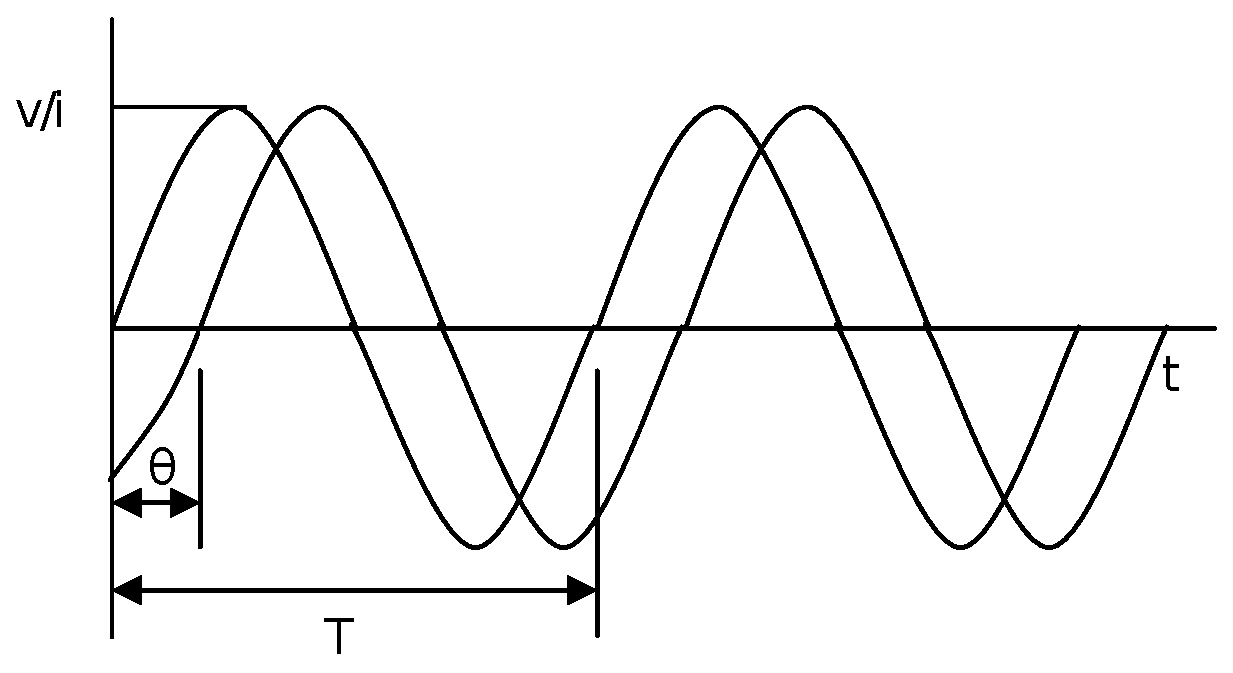
\includegraphics[width=0.6\textwidth]{img/acwave}
    \caption{Two Sinusoidal Waves With Phase Difference}
    \label{acwave}
  \end{figure}

  \begin{figure}[p]
    % ``Review of 3-Phase AC Circuits''  Not sure the university, but class
    % listed as EE340.  Author Y. Baghzouz.
    \centering
    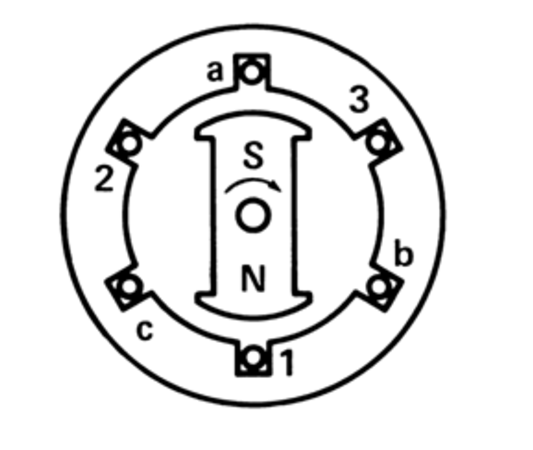
\includegraphics[width=0.4\textwidth]{img/threephasemotor}
    \caption{Simple Diagram of a Three-Phase Alternator}
    \label{alternator}
  \end{figure}

  \begin{figure}[p]
    \centering
    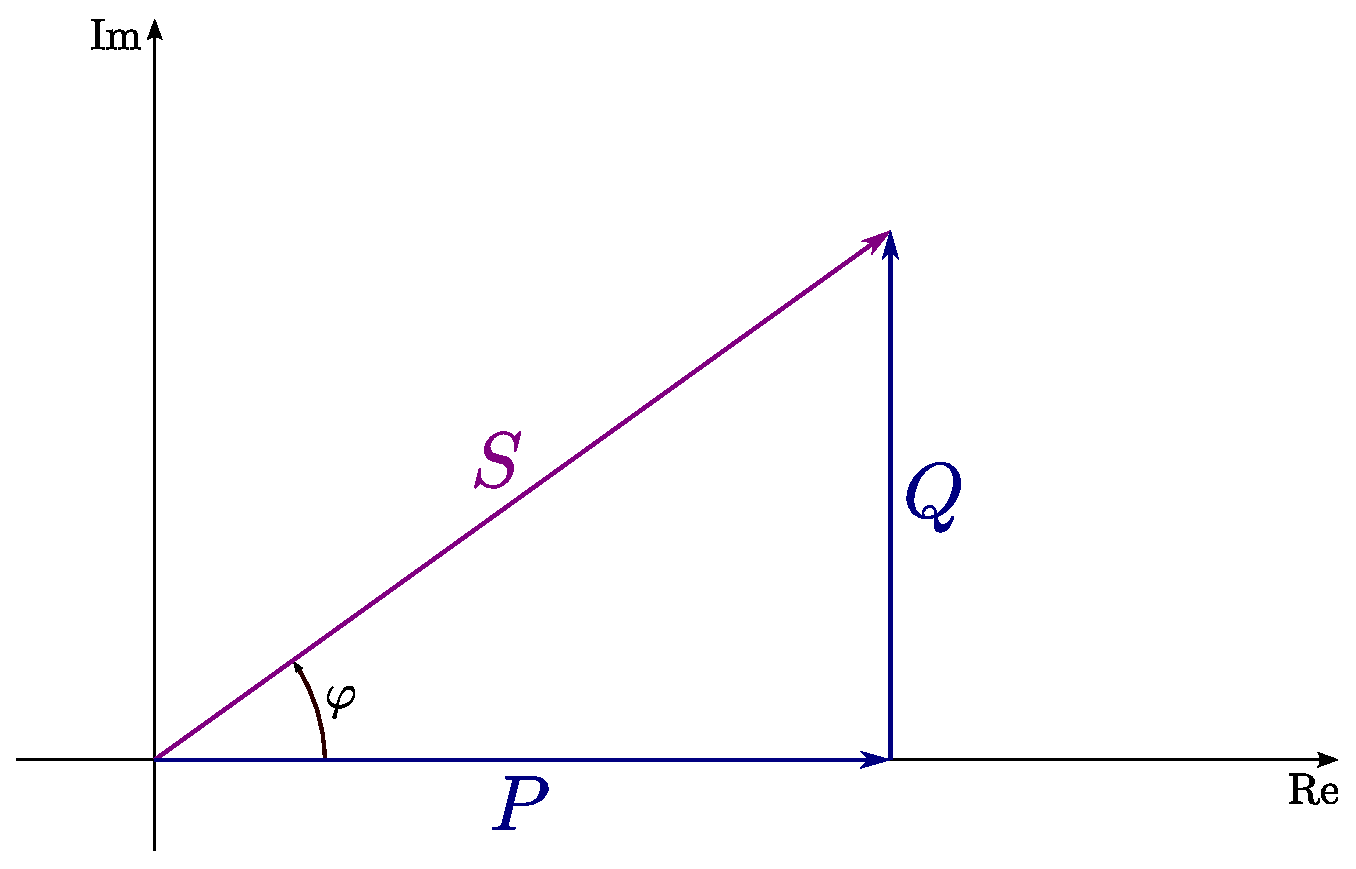
\includegraphics[width=0.5\textwidth]{img/complexpwr}
    \caption{Complex Power Triangle}
    \label{complexpwr}
  \end{figure}

\end{document}
